\chapter{Background}
\label{chap:background}

\section{Database Management Systems}
\label{sec:bg-dbms}

A database management system (DBMS) is software that stores and manages data based on a database model~\citep{dbms-wiki}. Among the various models, the relational model is the most widely adopted: data is organized into tables, where each row represents a record and each column represents an attribute~\citep{dbms-wiki}. Structured Query Language (SQL) is a domain-specific language used to create, query, and modify data in relational DBMSs~\citep{sql-standard}. In practice, although hundreds of DBMSs have been developed~\citep{dbengines}, each one extends or deviates from the SQL standard in different ways, resulting in dialect-specific syntax and behavior~\citep{sqlancer}.

In this thesis, we focus on SQLite as the target DBMS. SQLite is a self-contained, serverless database engine embedded directly into the host application, written in approximately 150{,}000 lines of C code~\citep{sqlite}. It is deployed in every major smartphone operating system, web browser, and the Python standard library, making it one of the most widely used software components in the world~\citep{sqlite}. Despite its maturity and extensive testing, SQLite has had memory safety vulnerabilities in deep subsystems such as the expression evaluator, the window function engine, and the generated column processor, which are the focus of our fuzzing campaigns.


\section{SQL Grammar}
\label{sec:bg-sql-grammar}

SQL grammar describes the syntax and semantic features of the SQL language~\citep{griffin}. SQL statements are the basic units that a DBMS receives and processes; they are defined by the grammar rules of the particular DBMS dialect. Although all relational DBMSs support a common core of SQL functionality, their grammars differ in practice. For example, the \texttt{CREATE TRIGGER} statement exists in SQLite, MariaDB, and PostgreSQL, but each DBMS uses a different syntax: SQLite uses \texttt{WHEN} clauses with \texttt{UPDATE} statements, MariaDB supports both \texttt{WHEN}-style triggers and \texttt{IF-THEN} conditional blocks, and PostgreSQL requires declaring a separate function~\citep{griffin}. These dialect differences mean that a grammar written for one DBMS cannot be directly reused for another.

For grammar-based fuzzing, the SQL grammar serves as the specification that guides input generation. By formally modeling the grammar, a fuzzer can systematically produce syntactically valid SQL statements that pass the DBMS parser and reach the deeper execution stages where vulnerabilities reside. Section~\ref{sec:bg-cfg} introduces the formal framework --- context-free grammars --- used to represent such grammars.


\section{Context-Free Grammars}
\label{sec:bg-cfg}

Programs that process structured input, such as SQL interpreters, cannot be effectively tested by methods that operate on raw bytes, because random byte sequences almost never produce syntactically valid inputs~\citep{nautilus}. Context-free grammars (CFGs) provide a formalism to specify the structure of such input languages, enabling the systematic generation of valid inputs~\citep{hopcroft}.

Intuitively, a CFG is a set of production rules where each rule specifies how a non-terminal symbol can be replaced by a sequence of terminal and non-terminal symbols. A special start non-terminal defines where derivation begins. The language described by a CFG is the set of all terminal strings that can be derived by repeatedly applying rules starting from the start symbol~\citep{hopcroft}.

More formally, a CFG is defined as a tuple $G = (N, T, R, S)$ where~\citep{hopcroft}:

\begin{itemize}
    \item $N$ is a finite set of \textit{non-terminal} symbols, representing intermediate states of the language specification.
    \item $T$ is a finite set of \textit{terminal} symbols, disjoint from $N$.
    \item $R$ is a finite set of \textit{production rules} of the form $A \to \alpha$ where $A \in N$ and $\alpha \in (T \cup N)^*$.
    \item $S \in N$ is the \textit{start symbol}. Every string generated by the CFG must be derivable from $S$.
\end{itemize}

Since the left-hand side of each rule consists of exactly one non-terminal, the possible derivations depend only on that non-terminal and not on the surrounding context --- hence the name \textit{context free}~\citep{hopcroft}.

To derive a string, a matching production rule is applied to the start symbol $S$. As long as the resulting sequence contains non-terminals, another rule is selected and applied to one of them. This process continues until only terminal symbols remain. Consider the following grammar fragment that generates simple SQL queries, written in the Nautilus Python DSL:

\begin{lstlisting}[language=Python, caption={A grammar fragment for SQL in the Nautilus Python DSL. Non-terminals are enclosed in curly braces. Each \texttt{ctx.rule} call defines one production rule.}, label={lst:sql-grammar}]
ctx.rule("Stmt", "SELECT {Expr} FROM {Table}")  # (1)
ctx.rule("Stmt", "{Stmt}; {Stmt}")               # (2)
ctx.rule("Expr", "{Col}")                         # (3)
ctx.rule("Expr", "{Func}({Expr})")                # (4)
ctx.rule("Table", "t1")                           # (5)
ctx.rule("Func", "printf")                        # (6)
ctx.rule("Col", "c1")                             # (7)
\end{lstlisting}

Starting from \texttt{Stmt}, one possible derivation applies rules in sequence:

\begin{center}
\texttt{Stmt} $\xrightarrow{(1)}$ \texttt{SELECT \{Expr\} FROM \{Table\}} $\xrightarrow{(4)}$ \texttt{SELECT \{Func\}(\{Expr\}) FROM \{Table\}} $\xrightarrow{(6)}$ \texttt{SELECT printf(\{Expr\}) FROM \{Table\}} $\xrightarrow{(3)}$ \texttt{SELECT printf(\{Col\}) FROM \{Table\}} $\xrightarrow{(7)}$ \texttt{SELECT printf(c1) FROM \{Table\}} $\xrightarrow{(5)}$ \texttt{SELECT printf(c1) FROM t1}
\end{center}

Each string generated by a CFG can be represented by its \textit{derivation tree}: the root is labeled with the start symbol, each internal node is a non-terminal, and the children of each node correspond to the right-hand side of the applied rule~\citep{hopcroft}. Leaf nodes are terminals. The generated string is obtained by reading leaves left to right --- a process called \textit{unparsing} in the context of grammar-based fuzzing~\citep{nautilus}. Figure~\ref{fig:derivation-tree} shows the derivation tree for the example above.

\begin{figure}[htbp]
\centering
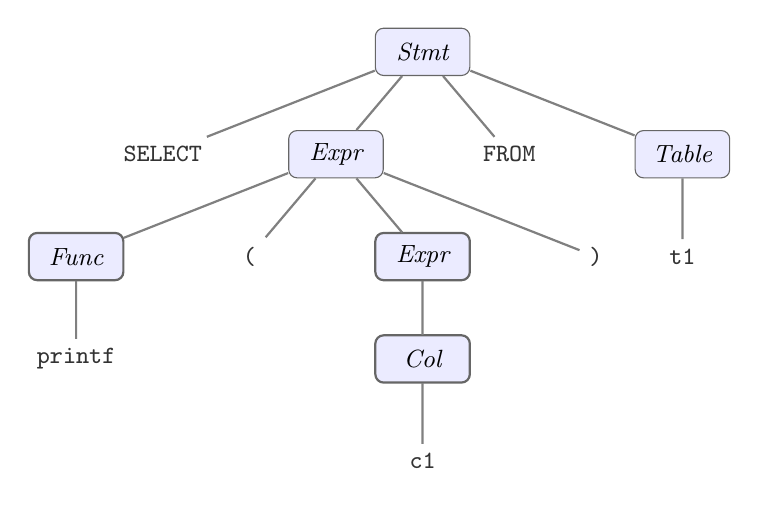
\begin{tikzpicture}[
    level distance=1.3cm,
    sibling distance=2.2cm,
    every node/.style={font=\small},
    nonterminal/.style={rectangle, rounded corners=3pt, draw=black!60,
        fill=blue!8, minimum width=1.2cm, minimum height=0.6cm,
        align=center, font=\small\itshape},
    terminal/.style={font=\small\ttfamily, text=black!80},
    edge from parent/.style={draw=black!50, thick},
]
\node[nonterminal] {Stmt}
    child { node[terminal] {SELECT} }
    child { node[nonterminal] {Expr}
        child { node[nonterminal] {Func}
            child { node[terminal] {printf} }
        }
        child { node[terminal] {(} }
        child { node[nonterminal] {Expr}
            child { node[nonterminal] {Col}
                child { node[terminal] {c1} }
            }
        }
        child { node[terminal] {)} }
    }
    child { node[terminal] {FROM} }
    child { node[nonterminal] {Table}
        child { node[terminal] {t1} }
    };
\end{tikzpicture}
\caption{Derivation tree for the SQL query \texttt{SELECT printf(c1) FROM t1}, generated from the grammar in Listing~\ref{lst:sql-grammar}. Internal nodes (rounded boxes) are non-terminals; leaf nodes are terminal symbols.}
\label{fig:derivation-tree}
\end{figure}

The key property for fuzzing is that every string derivable from a well-designed SQL grammar is a syntactically valid SQL statement. By designing the grammar to cover relevant SQL constructs, the generation process is guaranteed to produce inputs that pass the DBMS parser and reach deeper execution stages where vulnerabilities reside.


\section{Fuzzing}
\label{sec:bg-fuzzing}

Fuzzing is an automated technique for discovering software vulnerabilities by generating a large number of inputs, feeding them to a target program, and monitoring for abnormal behavior such as crashes or sanitizer violations~\citep{fuzzingsurvey}. In recent years, fuzzing has been applied extensively to test DBMSs and has found a large number of vulnerabilities~\citep{griffin}.

\paragraph{DBMS fuzzing.}
Unlike fuzzing C libraries that process binary formats, generating high-quality inputs for DBMSs is challenging because DBMSs enforce strict checks on both syntax and semantics~\citep{griffin}. A DBMS first checks the syntactic correctness of a SQL statement; incorrect statements are rejected outright. It then checks the semantics --- for example, whether referenced table and column names actually exist in the database. Statements that fail either check are discarded before reaching the deeper execution logic where vulnerabilities reside~\citep{griffin}.

DBMS fuzzers can be broadly categorized as generation-based or mutation-based~\citep{griffin}. Generation-based fuzzers construct SQL statements from a formal model of the grammar, such as an abstract syntax tree (AST). For example, SQLsmith~\citep{sqlsmith} introspects the database schema to generate type-correct queries, and SQLancer~\citep{sqlancer} generates queries designed to detect logic bugs through differential oracles. Mutation-based fuzzers modify existing SQL statements to produce new test cases, typically building a custom SQL parser and AST mutator for each target DBMS dialect. Squirrel~\citep{squirrel}, for instance, parses SQL into an intermediate representation that preserves semantic relationships, enabling type-aware mutations with coverage feedback.

\paragraph{Coverage-guided greybox fuzzing.}
A central insight of modern fuzzing is the use of code coverage as feedback to guide input generation. Coverage-guided greybox fuzzing, pioneered by AFL~\citep{afl}, instruments the target program to record which code edges (basic block transitions) are exercised during execution. The coverage information is stored in a shared memory bitmap. After executing a test input, the fuzzer checks whether any previously unseen edges were discovered; if so, the input is retained in the corpus for further mutation, otherwise it is discarded~\citep{fuzzingsurvey}. This feedback loop transforms fuzzing from random input generation into a directed search that progressively explores deeper program logic.

The AFL fork server model provides an efficient execution mechanism: rather than creating a new process for each test input, the target program is loaded once, and child processes are created via \texttt{fork()} for each test case. The child inherits the initialized program state, executes the input, and exits. This amortizes startup overhead and isolates crashes --- when a child triggers a fault, the parent remains unaffected~\citep{afl}.

\paragraph{Grammar-based greybox fuzzing.}
General-purpose greybox fuzzers such as AFL are effective for binary formats but struggle with structured inputs like SQL, because random byte-level mutations overwhelmingly produce parser-rejected inputs~\citep{nautilus}. Grammar-based fuzzing addresses this by generating inputs from a context-free grammar (Section~\ref{sec:bg-cfg}), ensuring syntactic validity. Combining grammar-based generation with coverage-guided feedback yields a \textit{grammar-based greybox fuzzer}: a system that generates syntactically valid inputs and uses coverage feedback to steer generation toward unexplored program regions. Nautilus~\citep{nautilus} is the first fuzzer to implement this combination, maintaining a corpus of derivation trees rather than flat strings and applying tree-level mutations guided by edge coverage. Nautilus discovered 13 previously unknown bugs across four interpreter targets (mruby, PHP, ChakraCore, and Lua), of which six were assigned CVEs, demonstrating that the grammar-plus-feedback combination significantly outperforms either approach alone.


\section{Related Work}
\label{sec:bg-related}

Several lines of research address the challenge of testing software that processes structured inputs. This section reviews the most relevant approaches and positions DBMS-Nautilus relative to each.

\paragraph{Generation-based fuzzers.}
CSmith~\citep{csmith} generates random C programs that avoid undefined behavior, enabling differential testing across compilers. CSmith demonstrates that grammar-driven generation can discover deep bugs that mutation-based tools miss, but it operates without coverage feedback: each generated program is independent of all previous executions. LangFuzz~\citep{langfuzz} combines grammar-based generation with code fragments parsed from an existing corpus to fuzz JavaScript interpreters, producing inputs that are both syntactically valid and semantically plausible. However, LangFuzz requires a pre-existing corpus and does not use coverage feedback. IFuzzer~\citep{ifuzzer} applies genetic programming to evolve JavaScript programs that maximize coverage, but evaluates fitness per generation rather than per input. Skyfire~\citep{skyfire} learns a probabilistic context-sensitive grammar from seed inputs and uses it to generate diverse seeds for downstream fuzzers, serving as a seed generator rather than a standalone fuzzer.

\paragraph{DBMS-specific testing tools.}
SQLsmith~\citep{sqlsmith} generates random SQL queries by introspecting database schema metadata, producing type-correct queries with valid table and column references. However, SQLsmith operates without coverage feedback and without weighted sampling over its query templates. Squirrel~\citep{squirrel} introduces an intermediate representation for SQL that encodes semantic relationships, enabling type-aware mutations with coverage feedback. However, Squirrel requires a custom IR parser for each SQL dialect and does not support weighted sampling over structural patterns. SQLancer~\citep{sqlancer} takes a different approach: rather than searching for crashes, it generates queries and checks whether the DBMS returns correct results. NoREC~\citep{norec} and TLP~\citep{tlp} extend this differential testing methodology. These tools are effective at detecting logic bugs (incorrect query results) but do not target memory safety violations, which require a crash-based oracle.

\paragraph{Grammar-based greybox fuzzers.}
Nautilus~\citep{nautilus} combines grammar-based generation with coverage-guided feedback in a closed loop, maintaining derivation trees as its internal representation and applying tree-level mutations. It discovered 13 bugs (six assigned CVEs) across four interpreter targets and demonstrated that the grammar-plus-feedback combination significantly outperforms either approach alone. However, Nautilus uses a general-purpose grammar with uniform sampling: all production rules have equal probability, with no mechanism to bias generation toward specific vulnerability classes.

\paragraph{Positioning of DBMS-Nautilus.}
DBMS-Nautilus extends the Nautilus architecture with three domain-specific enhancements. First, the grammar is designed around structural primitives extracted from CVE root-cause analysis, encoding the SQL constructs that stress vulnerability-prone code paths. Second, production rules carry numeric weights that bias sampling toward vulnerability-relevant constructs. Third, the grammar generates self-contained SQL programs from an empty database, eliminating the need for a pre-populated schema. Table~\ref{tab:related-comparison} summarizes the key differences.

\begin{table}[htbp]
\caption{Comparison of DBMS-Nautilus with related fuzzing tools. A checkmark indicates the tool supports the feature; a cross indicates it does not. ``SQL-specific'' indicates whether the tool is specifically designed for SQL or DBMS testing.}
\label{tab:related-comparison}
\centering
\small
\begin{tabular}{lccccc}
\toprule
\textbf{Tool} & \textbf{Grammar} & \textbf{Feedback} & \textbf{Corpus-free} & \textbf{SQL-specific} & \textbf{Weighted} \\
\midrule
AFL~\citep{afl}           & $\times$ & \checkmark & $\times$ & $\times$ & $\times$ \\
CSmith~\citep{csmith}     & \checkmark & $\times$ & \checkmark & $\times$ & $\times$ \\
SQLsmith~\citep{sqlsmith}  & \checkmark & $\times$ & $\times$ & \checkmark & $\times$ \\
Squirrel~\citep{squirrel}  & \checkmark & \checkmark & $\times$ & \checkmark & $\times$ \\
Nautilus~\citep{nautilus}  & \checkmark & \checkmark & \checkmark & $\times$ & $\times$ \\
DBMS-Nautilus             & \checkmark & \checkmark & \checkmark & \checkmark & \checkmark \\
\bottomrule
\end{tabular}
\end{table}
